\documentclass[12pt,spanish]{article}

% aprovechamiento de la p\'agina -- fill an A4 (210mm x 297mm) page

% Note: 1 inch = 25.4 mm = 72.27 pt
% 1 pt = 3.5 mm (approx)

\usepackage[paperheight=297mm,
            paperwidth=210mm,
            tmargin=28mm, 
            headheight=0mm, 
            headsep=0mm,
            textheight=240mm,
            footskip=7mm,
            textwidth=159.2mm,
            bindingoffset=10mm,
            twoside
            ]{geometry}

% paragraph setup
\setlength{\parindent}{0em}
%\setlength{\parindent}{4em}
\setlength{\parskip}{1em}
\setlength{\columnsep}{1em}
%\renewcommand{\baselinestretch}{1.5}

\usepackage{babel}
\usepackage[utf8]{inputenc}
\usepackage{amsmath,amsthm,mathtools,latexsym}
\usepackage{amsfonts,amssymb}
% \usepackage{amsmath,amsthm,mathtools}
% \usepackage{amsfonts,amssymb,latexsym,MnSymbol}
\usepackage{enumerate}
\usepackage[pdftex]{graphicx}
\usepackage[usenames,dvipsnames]{xcolor}
\usepackage[bookmarks=true,
            bookmarksnumbered=false, % true means bookmarks in 
                                     % left window are numbered                         
            bookmarksopen=false,     % true means only level 1
                                     % are displayed.
            colorlinks=true,
            linkcolor=webred]{hyperref}
\definecolor{webgreen}{rgb}{0, 0.5, 0} % less intense green
\definecolor{webblue}{rgb}{0, 0, 0.5}  % less intense blue
\definecolor{webred}{rgb}{0.5, 0, 0}   % less intense red
\definecolor{dkgreen}{rgb}{0,0.6,0}
\definecolor{gray}{rgb}{0.5,0.5,0.5}
\definecolor{mauve}{rgb}{0.58,0,0.82}
\definecolor{MistyRose}{RGB}{255,228,225}
\definecolor{LightCyan}{RGB}{224,255,255}
% Cambio de tipo de letra en entorno matemático

\usepackage[math]{iwona}
\usepackage{eulervm}
\usepackage[T1]{fontenc}
% \usepackage{beton}
% \usepackage[T1]{fontenc}

\usepackage{bigints}

% Theorem environments

%% \theoremstyle{plain} %% This is the default
\newtheorem{theorem}{Teorema}[section]
\newtheorem{corollary}[theorem]{Corolario}
\newtheorem{lemma}[theorem]{Lema}
\newtheorem{proposition}[theorem]{Proposici\'on}
\newtheorem{example}[theorem]{Ejemplo}
\newtheorem{exercise}[theorem]{Ejercicio}
\newtheorem{axiom}{Axioma}
\newtheorem{algoritmo}[theorem]{Algoritmo}

\theoremstyle{definition}
\newtheorem{definition}{Definici\'on}[section]
\theoremstyle{remark}
\newtheorem{remark}{Observaci\'on}[section]
\newtheorem*{notation}{Notaci\'on}
%\numberwithin{equation}{section}
\newcommand{\theoremref}[1]{Theorem~\ref{#1}}
\newcommand{\secref}[1]{\S\ref{#1}}
\newcommand{\lemmaref}[1]{Lemma~\ref{#1}}
%\newcommand{\bysame}{\mbox{\rule{3em}{.4pt}}\,}

%\pagestyle{empty}

\newcommand{\HRule}{\rule{\linewidth}{1mm}}
\title
{
\HRule
\begin{flushright}
\huge
\textbf{La Fórmula}\\
\Large
\textbf{de}\\
\Huge
\textbf{Bailey-Borwein-Plouffe}\\
\end{flushright}
\HRule 
} 
\author{\large \href{https://is.gd/xdhiYD}{Wikipedia}}
%\date{}

\begin{document}

\maketitle

%%% Local Variables: 
%%% mode: latex
%%% TeX-master: "bbp_formula"
%%% End:

\begin{abstract}
  \noindent
  En este artículo se desmuestra la fórmula BBP y se explica cómo
  calcular con ella dígitos calcular el enésimo dígito de $\pi$ en
  base $2$ (ó $16$) sin necesidad de hallar los precedentes.
\end{abstract}

\tableofcontents

%\setcounter{section}{-1}

\bibliographystyle{plain}

\section{Introducción}

Una cadena oruga es un dispositivo de desplazamiento utilizado
principalmente en vehículos pesados, como tanques y tractores, u otro
tipo de vehículos.\footnote{Como veremos no sólo (con acento, para que
  se chinche la RAE) los vehículos oruga eran vehículos pesados. Hubo
  moto--oruga que incluso se llegaron a usar en Alemania para
  posicionar los aviones en la pista de despege, evitando así que
  arrancasen sus motores antes de tiempo con el consiguiente ahorro de
  combustible.} Consiste en un conjunto de eslabones modulares que
permiten un desplazamiento estable aun en terrenos irregulares.

\begin{figure}[!hbp]
\centering
\mbox{
\subfigure[moto tractora]{
\label{mt}
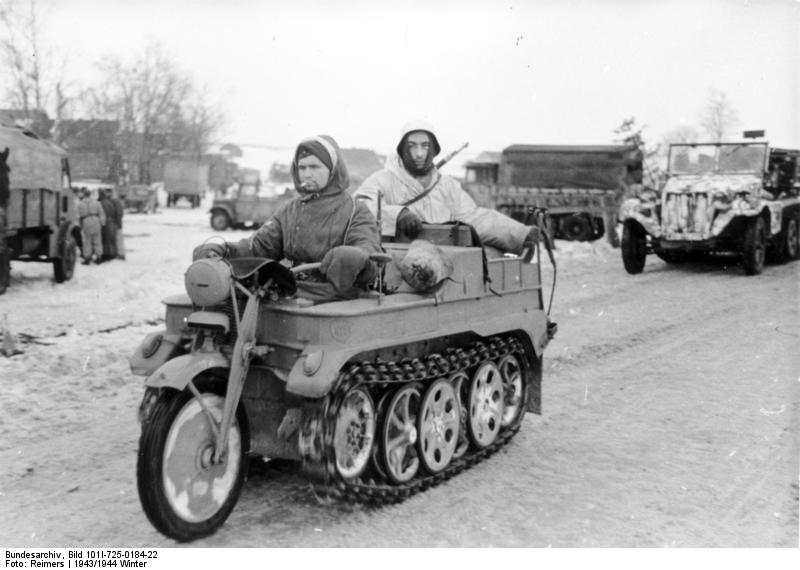
\includegraphics[width=.40\textwidth]{moto_tractora_orig.jpg}
}
\qquad
\subfigure[vehículo militar mixto]{
\label{vmm}
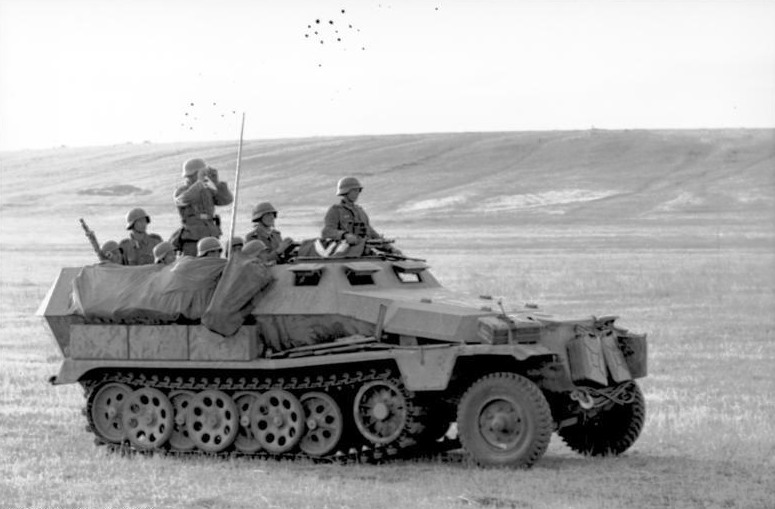
\includegraphics[width=.42\textwidth]{mixto.jpg}
}
}
\caption{\label{fig:militar} La oruga en el uso militar.}
\end{figure}

La {\it mayoría} de las \textit{orugas} forman parte de un
\emph{cinturón} flexible con un conjunto de eslabones rígidos unidos
unos a otros fuertemente. Los eslabones ayudan al vehículo a
distribuir el peso en una superficie mayor que la que hubiera tenido
con el empleo de ruedas, y esto hace que pueda moverse por un número
mayor de superficies sin hundirse debido a su propio peso. Por
ejemplo, la presión que ejerce un automóvil sobre el suelo es igual
aproximadamente a 207 kPa, mientras que las setenta toneladas que pesa
un carro M1 Abrams ejercen una presión sobre el firme de 103 kPa.

\begin{example}
  ~
  \begin{enumerate}
  \item Los tractores con una pala delante son los denominados
    bulldozers, y suelen ser usados en la construcción para remover
    tierra.
  \item Diversos vehículos incorporan la oruga en su mecánica de desplazamiento:
    \begin{enumerate}
    \item Carros de combate.
    \item Ciertos todoterreno de propósito específico, sobre todo de
      uso militar.
    \item Vehículos para el transporte por nieve e hielo.
    \end{enumerate}
  \item El transbordador espacial se transporta a su base de
    lanzamiento mediante una gran oruga transportadora.
  \item El vehículo con oruga más grande del mundo es la rotopala alemana Bagger 288.
  \end{enumerate}
\end{example}
%%% Local Variables: 
%%% mode: latex
%%% TeX-master: "bbp_formula"
%%% End:

\section{Demostración de la Fórmula BBP}

\begin{lemma}
  Para todo número natural $n$ se cumple:
  \begin{equation*}
    \sum_{k=0}^{\infty}\frac{1}{16^{k}(8k+n)}
    =\sqrt{2}^{n}\int_{0}^{\frac{1}{\sqrt{2}}}
    \left(\frac{x^{n-1}}{1-x^{8}}\right)
    \,dx
  \end{equation*}
\end{lemma}

\begin{proof}
  Sea $n$ un número natural cualquiera. Entonces:
  \begin{align*}
    \sum_{k=0}^{\infty}\frac{1}{16^{k}(8k+n)}
         &=\sqrt{2}^{n}\sum_{k=0}^{\infty}
             \frac{\left(\frac{1}{\sqrt{2}}\right)^{8k+n}}{8k+n}\\
         &=\sqrt{2}^{n}\sum_{k=0}^{\infty}
             \left[\frac{x^{8k+n}}{8k+n}\right]_{0}^{\frac{1}{\sqrt{2}}}\\
         &=\sqrt{2}^{n}\sum_{k=0}^{\infty}
           \left(
             \int _{0}^{\frac{1}{\sqrt{2}}}x^{8k+n-1}\,dx
           \right)\\
         &=\sqrt{2}^{n}\int _{0}^{\frac{1}{\sqrt{2}}}
           \left(\sum_{k=0}^{\infty}
                  x^{8k+n-1}
           \right)\,dx\\
         &=\sqrt{2}^{n}\int _{0}^{\frac{1}{\sqrt{2}}}
           \left(x^{n-1}\sum_{k=0}^{\infty}
                  (x^{8})^{k}
           \right)\,dx\\
             &=\sqrt{2}^{n}\int _{0}^{\frac{1}{\sqrt{2}}}
           \left(x^{n-1}\frac{1}{1-x^{8}}
           \right)\,dx\\
  \end{align*}
  
\end{proof}

\begin{theorem}
  Es cierta la siguiente igualdad (denominada
  \hyperref[eq:bbp]{fórmula BBP}):
  \begin{equation}
    \label{eq:bbp}
        \pi = \sum_{k=0}^{\infty}\frac{1}{16^{k}}
    \left(
      \frac{4}{8k+1}
      -\frac{2}{8k+4}
      -\frac{1}{8k+5}
      -\frac{1}{8k+6}
    \right) \nonumber
  \end{equation}
\end{theorem}

\begin{proof}
  Son ciertas las siguientes igualdades:
  \begin{align*}
    &\sum_{k=0}^{\infty}\frac{1}{16^{k}}
    \left(
      \frac{4}{8k+1}
      -\frac{2}{8k+4}
      -\frac{1}{8k+5}
      -\frac{1}{8k+6}
    \right)\\
     &=
     4\sum_{k=0}^{\infty}\frac{1}{16^{k}(8k+1)}
    -2\sum_{k=0}^{\infty}\frac{1}{16^{k}(8k+4)}
     -\sum_{k=0}^{\infty}\frac{1}{16^{k}(8k+5)}
     -\sum_{k=0}^{\infty}\frac{1}{16^{k}(8k+6)}\\
     &=4\left(\sqrt{2}^{1}\int_{0}^{\frac{1}{\sqrt{2}}}\frac{x^{1-1}}{1-x^{8}}\,dx\right)
     -2\left(\sqrt{2}^{4}\int_{0}^{\frac{1}{\sqrt{2}}}\frac{x^{4-1}}{1-x^{8}}\,dx\right)
     -\left(\sqrt{2}^{5}\int_{0}^{\frac{1}{\sqrt{2}}}\frac{x^{5-1}}{1-x^{8}}\,dx\right)\\
     &-\left(\sqrt{2}^{6}\int_{0}^{\frac{1}{\sqrt{2}}}\frac{x^{6-1}}{1-x^{8}}\,dx\right)\\
     &=\int_{0}^{\frac{1}{\sqrt{2}}}\frac{4\sqrt{2}-8x^{3}-4\sqrt{2}x^{4}-8x^{5}}
                                     {1-x^{8}}\,dx\\
  \end{align*}
  Haremos ahora el cambio de variable:
  \begin{equation*}
    \begin{cases}
      y=x\sqrt{2}&\\
      dy=dx\sqrt{2}&
    \end{cases}
  \end{equation*}
  Sustituyendo resulta lo siguiente:
  \begin{align*}
    \int_{0}^{\frac{1}{\sqrt{2}}}\frac{4\sqrt{2}-8x^{3}-4\sqrt{2}x^{4}-8x^{5}}
                                     {1-x^{8}}\,dx
    &=\bigint\limits_{0}^{1}\left(
      \frac{4\sqrt{2}-\frac{8}{\sqrt{2}^{3}}y^{3}
      -\frac{4\sqrt{2}}{\sqrt{2}^{4}}y^{4}
      -\frac{8}{\sqrt{2}^{5}}y^{5}}
       {1-\frac{1}{\sqrt{2}^{8}}y^{8}}\right)\,\frac{dy}{\sqrt{2}}\\
    &=16\int_{0}^{1}\frac{4-2y^{3}-y^{4}-y^{5}}{16-y^{8}}\,dy\\
    &=16\int_{0}^{1}\frac{y-1}{(y^{2}-2y+2)(y^{2}-2)}\,dy\\
  \end{align*}
  Descomponiendo en fracciones simples:
  \begin{align*}
    &=\int_{0}^{1}\left(
       \frac{8-4y}{y^{2}-2y+2}+\frac{4y}{y^{2}-2}\right)\,dy\\[3mm]
    &=-2\int_{0}^{1}\frac{2y-2}{y^{2}-2y+2}\,dy
      +4\int_{0}^{1}\frac{1}{1+(y-1)^{2}}\,dy
      +2\int_{0}^{1}\frac{2y}{y^{2}-2}\,dy\\[3mm]
    &=-2[\ln(y^{2}-2y+2)]_{0}^{1}
     +4[\arctan(y-1)]_{0}^{1}
     +2[\ln(2-y^{2})]_{0}^{1}\\[3mm]
    &=-2\ln(1)+2\ln(1)+4\arctan(0)-4\arctan(-1)+2\ln(1)-2\ln(2)\\[3mm]
    &=4\arctan(1)\\[3mm]
    &=\pi
  \end{align*}
\end{proof}
%%% Local Variables: 
%%% mode: latex
%%% TeX-master: "bbp_formula"
%%% End:

\section{Uso de la Fórmula para Calcular los Decimales del Número
  $\boldsymbol{\pi}$}


A continuación se muestra el cálculo del enésimo dígito hexadecimal de
$\pi$. Primero se debe observar que el dígito ubicado en la posición
$N+1$ de $\pi$ en base $16$ es el mismo que el primer dígito
hexadecimal de $16^{N}\pi$. En efecto, como en la base $10$,
multiplicar un número en base $16$ por $16$ equivale a desplazar la
coma decimal un lugar hacia la derecha. De esta manera, multiplicando
por $16^{N}$ la coma se desplaza $N$ lugares hacia la derecha. El
problema original se reduce al cálculo del primer dígito de
$16^{N}\pi$. Usando la \hyperref[eq:bbp]{fórmula BBP }:
\begin{equation*}
  16^{N}\pi =\sum_{k=0}^{\infty}16^{N-k}
  \left(
    \frac{4}{8k+1}
    -\frac{2}{8k+4}
    -\frac{1}{8k+5}
    -\frac{1}{8k+6}
  \right) \nonumber
\end{equation*}
    
El cálculo de los primeros dígitos hexadecimales a la derecha de la
coma de este número no es sencillo por dos razones: el número es muy
grande y la suma es infinita.
  
\begin{definition}
  Sea $N$ un número natural no nulo y $a$ un número natural. Definimos
  $S_{N}(a)$, $A_{N}(a)$ y $B_{N}(a)$ por las siguientes igualdades:
  \begin{eqnarray*}
    S_{N}(a)&=&\sum_{k=0}^{\infty}\frac{16^{N-k}}{8k+a}\\
    A_{N}(a)&=&\sum_{k=0}^{N-1}\frac{16^{N-k}}{8k+a}\\
    B_{N}(a)&=&\sum_{k=N}^{\infty}\frac{16^{N-k}}{8k+a}\\
  \end{eqnarray*}
\end{definition}

\begin{remark}
  Para tódo número natural $N$ no nulo y todo número natural:
  \begin{equation*}
    S_{N}(a) = A_{N}(a)+B_{N}(a)
  \end{equation*}
\end{remark}


El cálculo de los primeros dígitos hexadecimales de $S_{N}(a)$
permitirá obtener los de $16^{N}\pi$, a través de la relación:
\begin{equation*}
  16^{N}\pi=4S_{N}(1)-2S_{N}(4)-S_{N}(5)-S_{N}(6)
\end{equation*}

\subsection{Cálculo de $\boldsymbol{B_{N}(a)}$}

Aunque $B_{N}(a)$ es una suma infinita, es muy fácil de calcular
porque sus términos son pequeños y decrecen rápidamente. En efecto:
\begin{itemize}
\item el prmer término de la suma es $b_{N}=1/(8N+a)$. Si se busca
  el enésimo dígito hexadecimal de $\pi$ (digamos, por ejemplo,
  $N=1000000000$), el primer término es mucho menor que $1$.
\item Además, cada término tiene un cero más a la derecha de la coma
  que el precedente, porque para $k\geq N$, $b_{k}>16b_{k+1}$:
  \begin{align*}
    \frac{b_{k}}{b_{k+1}}&=\frac{16^{N-k}}{16^{N-(k+1)}}\frac{8(k+1)+a}{8k+a}\\
                         &=16\left(1+\frac{8}{8k+a}\right) \longrightarrow 16^{+}
  \end{align*}
\end{itemize}

Finalmente, la suma $B_{N}(a)$ es de la forma (en el peor caso):
\begin{align*}
  B_{N}&=0,**********\ldots\\
       &+0,0*********\ldots\\
       &+0,00********\ldots\\
       &+0,000*******\ldots\\ 
\end{align*}

Por lo tanto, para obtener $B_{N}(a)$ con una precisión de $P$ cifras
detrás de la coma, es suficiente calcular los $P$ primeros términos de
la suma, agregándose algunos términos más para eviatar errores que
aparecen al realizar cálculos con valores aproximados. Así, se
calcula:
\begin{equation*}
  B_{N}'=\sum_{k=N}^{N+P+10}\frac{16^{N-k}}{8k+a} 
\end{equation*}
Como esta suma posee una pequeña cantidad de términos, el tiempo que
insume esta operación es insignificante para la computadora.

\subsection{Cálculo de $\boldsymbol{A_{N}(a)}$}

El problema para el cálculo de $A_{N}(a)$ es que los primeros términos
son muy grandes ($N$ cifras de base $16$ antes de la coma). Sin
embargo, al igual que las primeras cifras detrás de la coma, no
importa la parte entera, que también es grande. Por lo tanto, puede
``eliminarse'' usando aritmética modular.

Toda la dificultad se reduce a hallar la parte fraccionaria de
$16^{N-k}/(8k+a)$. Para ello realizamos la división entera de
$16^{N-k}$ entre $(8k+a)$. Sabemos que existen números enteros $q$
y $r$ tales que:
\begin{itemize}
\item $16^{N-k}=q(8k+a)+r$
\item $0\leq r<8k+a$
\end{itemize}
Por tanto:
\begin{equation*}
  \frac{16^{N-k}}{8k+a}=q+\frac{r}{8k+a}
\end{equation*}
siendo $r/(8k+a)<1$ y por tanto es la parte fraccionaria de
$16^{N-k}/(8k+a)$ y
\begin{equation*}
  \frac{r}{8k+a}=\frac{16^{N-k}\mod (8k+a)}{8k+a}
\end{equation*}

Utilizando el método de la exponenciación binaria,
$16^{N-k}\mod (8k+a)$ se calcula rápidamente (con un tiempo de
ejecución de $\operatorname{O}(\log_{2}(N-k))$.

\subsection{Conclusión}

Al fin y al cabo, para obtener los primeros dígitos de $\pi$ en base
$16$ (ó $2$) se deben calcular los primeros dígitos de:
\begin{equation*}
  \pi_{N}=4S_{N}'(1)-2S_{N}'(4)-S_{N}'(5)-S_{N}'(6)
\end{equation*}
donde
\begin{equation*}
  S_{N}'(a) = \sum_{k=0}^{N-1}\frac{16^{N-k}\mod (8k+a)}{8k+a}
  +\sum_{k=N}^{N+P+10}\frac{16^{N-k}}{8k+a}
\end{equation*}
%%% Local Variables: 
%%% mode: latex
%%% TeX-master: "bbp_formula"
%%% End:

\section{Complejidad del Método}

Para calcular el enésimo dígito de $\pi$ en base $16$ (ó el $4n$-ésimo
dígito en base2):

\subsection*{Complejidad Temporal}

\begin{itemize}
\item $B_{N}'(a)$; se calcula con complejidad lineal
  $\operatorname{O}(1)$
\item $A_{N}'(a)$; utilizando el método de la exponenciación binaria,
  sus términos se calculan en $\operatorname{O}(\log_{2}(n))$. Así la
  suma de $n$ términos, $A_{N}'(a)$, se calcula en
  $\operatorname{O}(n\log_{2}(n))$.
\end{itemize}
Así $S_{N}'(a)$ se calcula en 
\begin{equation*}
  \operatorname{O}(1)+\operatorname{O}(n\log_{2}(n))=
  \operatorname{O}(n\log_{2}(n))
\end{equation*}
Finalmente, $\pi_{n}$ se calcula en
\begin{equation*}
  4\operatorname{O}(n\log_{2}(n))=\operatorname{O}(n\log_{2}(n))    
\end{equation*}
Así pues, si el tiempo de cálculo es proporcional a $n\log_{2}(n)$,
es casi lineal.

\subsection*{Complejidad Espacial}

La complejidad en el uso de memoria es constante, ya que sólo se
realizan sumas sucesivas de pequeños números (con una precisión de
unos diez decimales es suficiente).
%%% Local Variables: 
%%% mode: latex
%%% TeX-master: "bbp_formula"
%%% End:

\section{Fórmulas Derivadas}

\begin{itemize}
\item   Fórmula original:
  \begin{equation*}
    \pi = \sum_{i=0}^{\infty}\frac{1}{16^{i}}
    \left(
      \frac{4}{8i+1}
      -\frac{2}{8i+4}
      -\frac{1}{8i+5}
      -\frac{1}{8i+6}
    \right)
  \end{equation*}
\item Para todo $r\in\mathbb{C}$:
  \begin{equation*}
    \pi = \sum_{i=0}^{\infty}\frac{1}{16^{i}}
    \left(
      \frac{4+8r}{8i+1}
      -\frac{8r}{8i+2}
      -\frac{4r}{8i+3}
      -\frac{2+8i}{8i+4}
      -\frac{1+2r}{8i+5}
      -\frac{1+2r}{8i+6}
      +\frac{r}{8i+7}
    \right)
  \end{equation*} 
\item Cáculo de $\pi\sqrt{2}$:
  \begin{equation*}
    \pi\sqrt{2} = \sum_{i=0}^{\infty}\frac{(-1)^{i}}{8^{i}}
    \left(
      \frac{4}{6i+1}
      +\frac{1}{6i+2}
      +\frac{1}{6i+3}
    \right)
  \end{equation*}
\item Expresión de $\pi^{2}$:
  \begin{align*}
    \pi^{2}= \sum_{i=0}^{\infty}\frac{1}{16^{i}}&
      \left(
        \frac{16}{(8i+1)^{2}}
        -\frac{16}{(8i+2)^{2}}
        -\frac{8}{(8i+3)^{2}}
        -\frac{16}{(8i+4)^{2}}
        -\frac{4}{(8i+5)^{2}}
        -\frac{4}{(8i+6)^{2}}\right.\\
        &\left.-\frac{2}{(8i+7)^{2}}\right)
  \end{align*}
\item Expresión de $\pi^{2}$:
  \begin{equation*}
    \pi^{2}=\frac{9}{8}\sum_{i=0}^{\infty}\frac{1}{64^{i}}
    \left(
      \frac{16}{(6i+1)^{2}}
      -\frac{24}{(6i+2)^{2}}
      -\frac{8}{(6i+3)^{2}}
      -\frac{6}{(6i+4)^{2}}
      -\frac{1}{(6i+5)^{2}}
    \right)
  \end{equation*}
\item La siguiente expresión permite hallar dígitos aislados de
  $\pi^{2}$ en base $3$ ó $9$:
  \begin{align*}
    \pi^{2}=\frac{2}{27}\sum_{i=0}^{\infty}\frac{1}{729^{i}}&
      \left(
        \frac{243}{(12i+1)^{2}}
        -\frac{405}{(12i+2)^{2}}
        -\frac{81}{(12i+4)^{2}}
        -\frac{27}{(12i+5)^{2}}
        -\frac{72}{(12i+6)^{2}}\right.\\
        &\left.-\frac{9}{(12i+7)^{2}}
        -\frac{9}{(12i+8)^{2}}
        -\frac{5}{(12i+10)^{2}}
        -\frac{1}{(12i+11)^{2}}
          \right)
  \end{align*}
\item Viktor Adamchick y Stan Wagon (1997):
  \begin{equation*}
    \pi = \sum_{i=0}^{\infty}\frac{(-1)^{i}}{4^{i}}
    \left(
      \frac{2}{4i+1}
      +\frac{2}{4i+2}
      +\frac{1}{4i+3}
    \right)
  \end{equation*}
\item Fabrice Bellard
  \begin{align*}
    \pi =\frac{1}{64}\sum_{i=0}^{\infty}\frac{(-1)^{i}}{2^{10i}}&
      \left(
        -\frac{32}{4i+1}
        -\frac{1}{4i+3}
        +\frac{256}{10i+1}
        -\frac{64}{10i+3}
        -\frac{4}{10i+5}
        -\frac{4}{10i+7}\right.\\
        &\left.+\frac{1}{10i+9}
          \right)
  \end{align*}
\end{itemize}
%%% Local Variables: 
%%% mode: latex
%%% TeX-master: "bbp_formula"
%%% End:

\section{Los Récords}

\begin{flushleft}
  Para poder comparar, hasta el año 2008 se habían obtenido los
  primeros $1,241$ billones de decimales de $\pi$ (aproximadamente
  $4,123$ billones de bits):
  \begin{itemize}
  \item 7 de octubre de 1996
    (\href{https://es.wikipedia.org/wiki/Fabrice_Bellard}{Fabrice
      Bellard}): dígito número $400$ mil millones en base $2$.
  \item septiembre de 1997
    (\href{https://es.wikipedia.org/wiki/Fabrice_Bellard}{Fabrice
      Bellard}): billonésimo dígito en base $2$.
  \item febrero de 1999 (Colin Percival): dígito número $40$ billones en
    base $2$
  \item 2001: dígito número $4000$ billones en base $2$
  \item 2011: dígito número $10$ billones en base $2$
  \end{itemize}
\end{flushleft}

\section{Cálculo del enésimo decimal}

\begin{flushleft}
  Actualmente, no existe ninguna fórmula eficaz para hallar el enésimo
  decimal de $\pi$ en base $10$. \textit{Simon Plouffe} ha
  desarrollado en diciembre de 1996, a partir de una serie muy antigua
  que calcula $\pi$ basado en los coeficientes de
  \href{https://es.wikipedia.org/wiki/Binomio_de_Newton}{binomio de
    Newton}, un método para calcular cifras aisladas base $10$, pero
  debido a su complejidad $\operatorname{O}(n^{3}\log_{2}(n))$ pierde
  su utilidad en la
  práctica. \href{https://es.wikipedia.org/wiki/Fabrice_Bellard}{Fabrice
    Bellard} ha mejorado el algoritmo para alcanzar un nivel de
  complejidad en $\operatorname{O}(n^{2})$, pero no es suficiente para
  competir con los métodos convencionales que calculan todos los
  decimales.
\end{flushleft}

\nocite{bai}

\bibliography{bbp_formula}

\end{document}